\chapter{Судалгааны арга зүй}
\label{ch:methodology}

\section{Системийн шинжилгээ ба шаардлага}
\label{sec:system_analysis}

\subsection{Арга зүйн хандлага}

Энэхүү ажлыг Дизайн шинжлэх ухааны судалгааны (Design Science Research, DSR) арга зүйгээр гүйцэтгэж, AI Notebook системийн шаардлага, хэрэгжилт, баталгаажуулалтыг нэг шугамд уялдуулсан \cite{hevner2004}\cite{peffers2007}.

Судалгааны хэрэгжилтийг дараах товч үе шаттайгаар зохион байгуулсан:

\begin{enumerate}
    \item Шаардлага ба архитектур тодорхойлох,
    \item Frontend/backend хэрэгжилт хийх,
    \item Интеграцийн урсгал ба өгөгдлийн урсгалын түвшний баталгаажуулалт хийх.
\end{enumerate}
\subsection{Шаардлагын тодорхойлолт}

Системийн хөгжүүлэлтийг хяналттай байлгахын тулд функционал болон функционал бус шаардлагуудыг (NFR) тусад нь тодорхойлж, аль шаардлага аль модульд хэрэгжсэн, хэрхэн баталгаажсан зэргийг мөрдөх матрицаар харуулав.

\begin{table}[H]
\centering
\caption{Функционал шаардлагын мөрдөх матриц}
\label{tab:functional_requirements_trace}
\small
\setlength{\tabcolsep}{4pt}
\renewcommand{\arraystretch}{1.15}
\begin{tabularx}{\textwidth}{>{\raggedright\arraybackslash}p{1.6cm}>{\raggedright\arraybackslash}X>{\raggedright\arraybackslash}p{3.6cm}>{\raggedright\arraybackslash}p{2.4cm}}
\toprule
\textbf{ID} & \textbf{Шаардлага} & \textbf{Хэрэгжүүлсэн модуль} & \textbf{Баталгаажуулалт} \\
\midrule
FR-1 & Бүртгэл/нэвтрэлт хийх & Auth API, Login/Signup дэлгэц & Signup/Login интеграцийн тест \\
FR-2 & Тэмдэглэл үүсгэх, шинэчлэх, устгах & Notes API, Dashboard/Calendar UI & CRUD туршилтын сценарууд \\
FR-3 & AI стикер үүсгэх & Sticker API, Sticker UI & \texttt{/generate-sticker} хүсэлтийн тест \\
FR-4 & Сануулга тохируулах ба мэдэгдэл авах & NotificationService, Notifications UI & Reminder scheduling шалгалт \\
FR-5 & Календарь дээр тэмдэглэл харах & Calendar UI, \texttt{noteDate} шүүлт & Огнооны шүүлтийн шалгалт \\
\bottomrule
\end{tabularx}
\normalsize
\end{table}

\begin{table}[H]
\centering
\caption{Функционал бус шаардлага (NFR) ба үнэлгээний хандлага}
\label{tab:nfr_requirements_trace}
\small
\setlength{\tabcolsep}{4pt}
\renewcommand{\arraystretch}{1.15}
\begin{tabularx}{\textwidth}{>{\raggedright\arraybackslash}p{1.8cm}>{\raggedright\arraybackslash}X>{\raggedright\arraybackslash}p{3.8cm}>{\raggedright\arraybackslash}p{2.2cm}}
\toprule
\textbf{ID} & \textbf{NFR агуулга} & \textbf{Инженерийн шийдэл} & \textbf{Үнэлгээний арга} \\
\midrule
NFR-1 & Аюулгүй байдал & JWT + middleware + secure storage & Token/401 баталгаажуулалт \\
NFR-2 & Найдвартай ажиллагаа & Алдааны боловсруулалт, fallback урсгал & Error scenario тест \\
NFR-3 & Хариу хугацааны хүлцэл & Async endpoint, latency хэмжилт & p50/p95, mean latency \\
NFR-4 & Засварлах чадвар & Route/controller тусгаарлалт & Модуль тусгаарлагдсан кодын бүтэц \\
NFR-5 & UX тогтвортой байдал & Snackbar feedback, state refresh & Үйлдлийн дараах UI шалгалт \\
\bottomrule
\end{tabularx}
\normalsize
\end{table}

\section{Системийн архитектур ба загварчлал}
\label{sec:system_design}

\subsection{Аппын бүрэн урсгалын диаграм} Зураг 4.1 нь апп нээгдэхээс эхлээд нэвтрэлт, тэмдэглэлийн удирдлага, AI стикер үүсгэх, өгөгдөл хадгалах, календарь болон мэдэгдлийн үндсэн урсгалыг нэгтгэн харуулна. \texttt{SplashRouter} нь токены төлөвөөр хэрэглэгчийг \texttt{LoginScreen} эсвэл \texttt{DashboardScreen} руу чиглүүлж, цааш тэмдэглэл үүсгэх/засах/устгах урсгал руу шилжүүлнэ. Үүссэн мэдээлэл \texttt{MongoDB}-д хадгалагдаж, \texttt{reminderAt}-д тулгуурлан календарь болон push notification-тэй уялдан ажиллана.

\begin{figure}[H]
\centering
\begin{tikzpicture}[
    scale=0.87,
    transform shape,
    %% ── Node styles ─────────────────────────────────────────────
    start/.style ={draw=black!70, line width=1.4pt, rounded corners=16pt,
                                 minimum width=3.8cm, minimum height=1.0cm,
                                 align=center, fill=gray!18, font=\small\bfseries},
    proc/.style  ={draw=blue!55, line width=1.2pt, rounded corners=6pt,
                                 minimum width=4.6cm, minimum height=1.0cm,
                                 align=center, fill=blue!8, font=\small},
    dec/.style   ={draw=orange!70, line width=1.4pt, diamond,
                                 minimum width=3.6cm, minimum height=1.4cm,
                                 align=center, fill=orange!12, font=\small\bfseries},
    login/.style ={draw=red!50, line width=1.2pt, rounded corners=6pt,
                                 minimum width=3.8cm, minimum height=1.0cm,
                                 align=center, fill=red!8, font=\small},
    note/.style  ={draw=blue!55, line width=1.2pt, rounded corners=6pt,
                                 minimum width=4.6cm, minimum height=1.1cm,
                                 align=center, fill=blue!8, font=\small},
    create/.style={draw=violet!60, line width=1.2pt, rounded corners=6pt,
                                 minimum width=4.6cm, minimum height=1.1cm,
                                 align=center, fill=violet!8, font=\small},
    ainod/.style ={draw=orange!70, line width=1.4pt, rounded corners=6pt,
                                 minimum width=4.6cm, minimum height=1.1cm,
                                 align=center, fill=orange!18, font=\small\bfseries},
    dbnod/.style ={draw=yellow!70!black, line width=1.2pt, rounded corners=6pt,
                                 minimum width=4.6cm, minimum height=1.1cm,
                                 align=center, fill=yellow!22, font=\small},
    calnod/.style={draw=green!60!black, line width=1.4pt, rounded corners=6pt,
                                 minimum width=4.6cm, minimum height=1.1cm,
                                 align=center, fill=green!15, font=\small\bfseries},
    fcm/.style   ={draw=red!60, line width=1.4pt, rounded corners=6pt,
                                 minimum width=4.6cm, minimum height=1.1cm,
                                 align=center, fill=red!10, font=\small\bfseries},
    grpblue/.style  ={draw=blue!40,   line width=0.8pt, dashed, rounded corners=8pt, fill=blue!4,   inner sep=8pt},
    grpred/.style   ={draw=red!40,    line width=0.8pt, dashed, rounded corners=8pt, fill=red!4,    inner sep=8pt},
    grpviolet/.style={draw=violet!40, line width=0.8pt, dashed, rounded corners=8pt, fill=violet!4, inner sep=8pt},
    grpgreen/.style ={draw=green!50!black, line width=0.8pt, dashed, rounded corners=8pt, fill=green!4, inner sep=8pt},
    arr/.style   ={-{Stealth[length=7pt]}, line width=1.2pt, color=black!60},
    lbl/.style   ={draw=none, fill=white, rounded corners=3pt,
                                 inner sep=2pt, font=\scriptsize\itshape, text=black!70}
]

    %% ── Nodes ──────────────────────────────────────────────────
    \node[start]  (appstart) at (0,    0   ) {Апп нээх};
    \node[proc]   (splash)   at (0,   -2.0 ) {SplashRouter};
    \node[dec]    (check)    at (0,   -4.4 ) {Токен бий юу?};

    \node[login]  (loginN)   at (-5.6, -6.8) {LoginScreen};
    \node[proc]   (dash)     at (0,   -6.8 ) {DashboardScreen};

    \node[note]   (list)     at (0,   -9.0 ) {Тэмдэглэл жагсаалт\\[-2pt]
                                                                                         {\scriptsize харах \textbullet\ засах \textbullet\ устгах}};
    \node[create] (create)   at (6.6, -9.0 ) {Шинэ тэмдэглэл\\[-2pt]
                                                                                         {\scriptsize текст + mood + огноо}};
    \node[ainod]  (ai)       at (6.6, -11.2) {\textbf{AI Sticker} үүсгэх\\[-2pt]
                                                                                         {\scriptsize mood шинжлэж стикер гаргана}};
    \node[dbnod]  (db)       at (6.6, -13.4) {MongoDB хадгалах\\[-2pt]
                                                                                         {\scriptsize reminderAt}};
    \node[calnod] (cal)      at (0,   -13.4) {\textbf{Calendar} харах\\[-2pt]
                                                                                         {\scriptsize стикер + огноо дээр харагдана}};
    \node[fcm]    (notif)    at (0,   -15.6) {\textbf{Push Notification}\\[-2pt]
                                                                                         {\scriptsize reminderAt болоход FCM автомат}};

    %% ── Group background boxes ──────────────────────────────────
    \begin{scope}[on background layer]
        \node[grpblue,   fit=(appstart)(splash)(check)] {};
        \node[grpred,    fit=(loginN)]                  {};
        \node[grpblue,   fit=(dash)(list)]              {};
        \node[grpviolet, fit=(create)(ai)(db)]          {};
        \node[grpgreen,  fit=(cal)(notif)]              {};
    \end{scope}

    %% ── Arrows ──────────────────────────────────────────────────
    \draw[arr] (appstart) -- (splash);
    \draw[arr] (splash)   -- (check);
    \draw[arr] (check.west) -| (loginN.north);
    \draw[arr] (check.south) -- (dash.north);
    \draw[arr] (loginN.east) -- (dash.west);
    \draw[arr] (dash)     -- (list);
    \draw[arr] (list.east) -- (create.west);
    \draw[arr] (create)   -- (ai);
    \draw[arr] (ai)       -- (db);
    \draw[arr] (db.west)  -- (cal.east);
    \draw[arr] (cal)      -- (notif);

\end{tikzpicture}
\caption{Апп-ын бүрэн үйл ажиллагааны урсгалын диаграм}
\label{fig:flowchart}
\end{figure}

\section{Ерөнхий ойлголтоос нарийвчилсан өгөгдлийн урсгалын зураг руу}

Энэ бүлгийн гол зорилго нь өгөгдлийн урсгалыг эхлээд \textbf{Зураг 4.2} (context level), дараа нь \textbf{Зураг 4.3} (level-1 dataflow), эцэст нь \textbf{Зураг 4.4--4.6} (level-2 dataflow) руу шаталж тайлбарлах юм. Харин \textbf{Зураг 4.1} нь апп-ын ерөнхий үйл ажиллагааны урсгалын нэгтгэлийг харуулна.



\begin{figure}[H]
\centering
\resizebox{0.95\textwidth}{!}{%
\begin{tikzpicture}[
    font=\small,
    ext/.style={rectangle, rounded corners=8pt, draw=blue!65, fill=blue!8, minimum width=3.9cm, minimum height=1.2cm, text width=3.6cm, align=center},
    proc/.style={rectangle, rounded corners=10pt, draw=purple!70, fill=purple!10, minimum width=5.6cm, minimum height=1.7cm, text width=5.0cm, align=center, font=\bfseries},
    store/.style={rectangle, rounded corners=8pt, draw=green!55!black, fill=green!9, minimum width=4.0cm, minimum height=1.2cm, text width=3.6cm, align=center},
    service/.style={rectangle, rounded corners=8pt, draw=black!60, fill=gray!12, minimum width=4.0cm, minimum height=1.2cm, text width=3.6cm, align=center},
    arr/.style={-Stealth, line width=1.05pt},
    lbl/.style={fill=white, inner sep=1pt, font=\scriptsize, align=center}
]

\node[ext] (user) at (-7.0,0) {Хэрэглэгч\\(мобайл интерфейс)};
\node[proc] (sys) at (0,0) {AI Notebook систем};
\node[store] (db) at (7.0,2.15) {MongoDB\\Хэрэглэгч/тэмдэглэл};
\node[service] (openai) at (7.0,-2.15) {OpenRouter API\\Зураг үүсгэх үйлчилгээ};

\draw[arr] ([yshift=6pt]user.east) -- node[above, lbl] {UI хүсэлт} ([yshift=6pt]sys.west);
\draw[arr] ([yshift=-6pt]sys.west) -- node[below, lbl] {Дэлгэц, мэдэгдэл} ([yshift=-6pt]user.east);

\draw[arr] ([yshift=12pt]sys.east) -- node[above, sloped, lbl] {CRUD хүсэлт} ([yshift=8pt]db.west);
\draw[arr] ([yshift=-6pt]db.west) -- node[below, sloped, lbl] {Query үр дүн} ([yshift=2pt]sys.east);

\draw[arr] ([yshift=-2pt]sys.east) -- node[above, sloped, lbl] {Prompt} ([yshift=6pt]openai.west);
\draw[arr] ([yshift=-8pt]openai.west) -- node[below, sloped, lbl] {Sticker URL} ([yshift=-12pt]sys.east);

\end{tikzpicture}%
}
\caption{Контекст түвшний өгөгдлийн урсгалын зураг}
\label{fig:dfd_context}
\end{figure}

\noindent \fref{fig:dfd_context}-д системийг нэг процесс гэж үзэж, гаднах оролцогчид (хэрэглэгч, OpenRouter API) болон өгөгдлийн сангийн харилцааг ерөнхий түвшинд харуулав.


\begin{figure}[H]
\centering
\begin{tikzpicture}[
    font=\small,
    proc/.style={rectangle, rounded corners=8pt, draw=purple!70, fill=purple!8, minimum width=4cm, minimum height=1.2cm, text width=3.8cm, align=center},
    ext/.style={rectangle, rounded corners=6pt, draw=blue!60, fill=blue!8, minimum width=3.2cm, minimum height=1.2cm, text width=3.0cm, align=center},
    store/.style={rectangle, rounded corners=6pt, draw=green!55!black, fill=green!8, minimum width=3.2cm, minimum height=1.2cm, text width=2.8cm, align=center},
    arr/.style={-Stealth, line width=1.05pt},
    lbl/.style={fill=white, inner sep=1.5pt, font=\scriptsize, align=center}
]

\node[ext]   (app) at (-6.8, 0) [minimum height=2.2cm] {Flutter аппликейшн\\(Flutter app)};

\node[proc]  (p1)  at (0, 3.8) {P1: Баталгаажуулалтын API\\(Auth API)};
\node[proc]  (p2)  at (0, 0) {P2: Тэмдэглэлийн API\\(Notes API)};
\node[proc]  (p3)  at (0, -3.8) {P3: Стикерийн API\\(Sticker API)};

\node[store] (d1)  at (6.8, 3.8) {D1: Хэрэглэгчид\\(Users)};
\node[store] (d2)  at (6.8, 0) {Тэмдэглэл\\(Notes)};
\node[ext]   (oa)  at (6.8, -3.8) {OpenRouter API};

% App <-> P1
\draw[arr] ([yshift=24pt]app.east) -- node[above, sloped, lbl] {Бүртгэл, нэвтрэх хүсэлт} ([yshift=6pt]p1.west);
\draw[arr] ([yshift=-6pt]p1.west) -- node[below, sloped, lbl] {Токен, хэрэглэгч} ([yshift=12pt]app.east);

% App <-> P2
\draw[arr] ([yshift=6pt]app.east) -- node[above, lbl] {GET/POST/\\PUT/DELETE} ([yshift=6pt]p2.west);
\draw[arr] ([yshift=-6pt]p2.west) -- node[below, lbl] {Тэмдэглэлийн\\JSON} ([yshift=-6pt]app.east);

% App <-> P3
\draw[arr] ([yshift=6pt]p3.west) -- node[above, sloped, lbl] {Sticker URL (Зураг)} ([yshift=-12pt]app.east);
\draw[arr] ([yshift=-24pt]app.east) -- node[below, sloped, lbl] {Заавар текст (prompt)} ([yshift=-6pt]p3.west);

% P1 <-> D1
\draw[arr] ([yshift=8pt]p1.east) -- node[above, lbl] {Шалгах,\\хадгалах} ([yshift=8pt]d1.west);
\draw[arr] ([yshift=-8pt]d1.west) -- node[below, lbl] {Хэрэглэгчийн\\мэдээлэл} ([yshift=-8pt]p1.east);

% P2 <-> D2
\draw[arr] ([yshift=8pt]p2.east) -- node[above, lbl] {CRUD үйлдэл} ([yshift=8pt]d2.west);
\draw[arr] ([yshift=-8pt]d2.west) -- node[below, lbl] {Өгөгдлийн\\үр дүн} ([yshift=-8pt]p2.east);

% P3 <-> OA
\draw[arr] ([yshift=8pt]p3.east) -- node[above, lbl] {Prompt\\дамжуулах} ([yshift=8pt]oa.west);
\draw[arr] ([yshift=-8pt]oa.west) -- node[below, lbl] {Зургийн\\холбоос} ([yshift=-8pt]p3.east);

\end{tikzpicture}
\caption{Нэгдүгээр түвшний өгөгдлийн урсгал: сервер талын модулийн задаргаа}
\label{fig:dfd_level1}
\end{figure}

\noindent \fref{fig:dfd_level1}-д системийн дотоод логикийг P1 (баталгаажуулалт), P2 (тэмдэглэлийн CRUD), P3 (AI стикер) гэсэн үндсэн процессуудад задалж, Flutter аппликейшн, MongoDB, OpenRouter API үйлчилгээтэй ямар өгөгдөл солилцож байгааг тодорхой түвшинд харуулсан.

\begin{figure}[H]
\centering
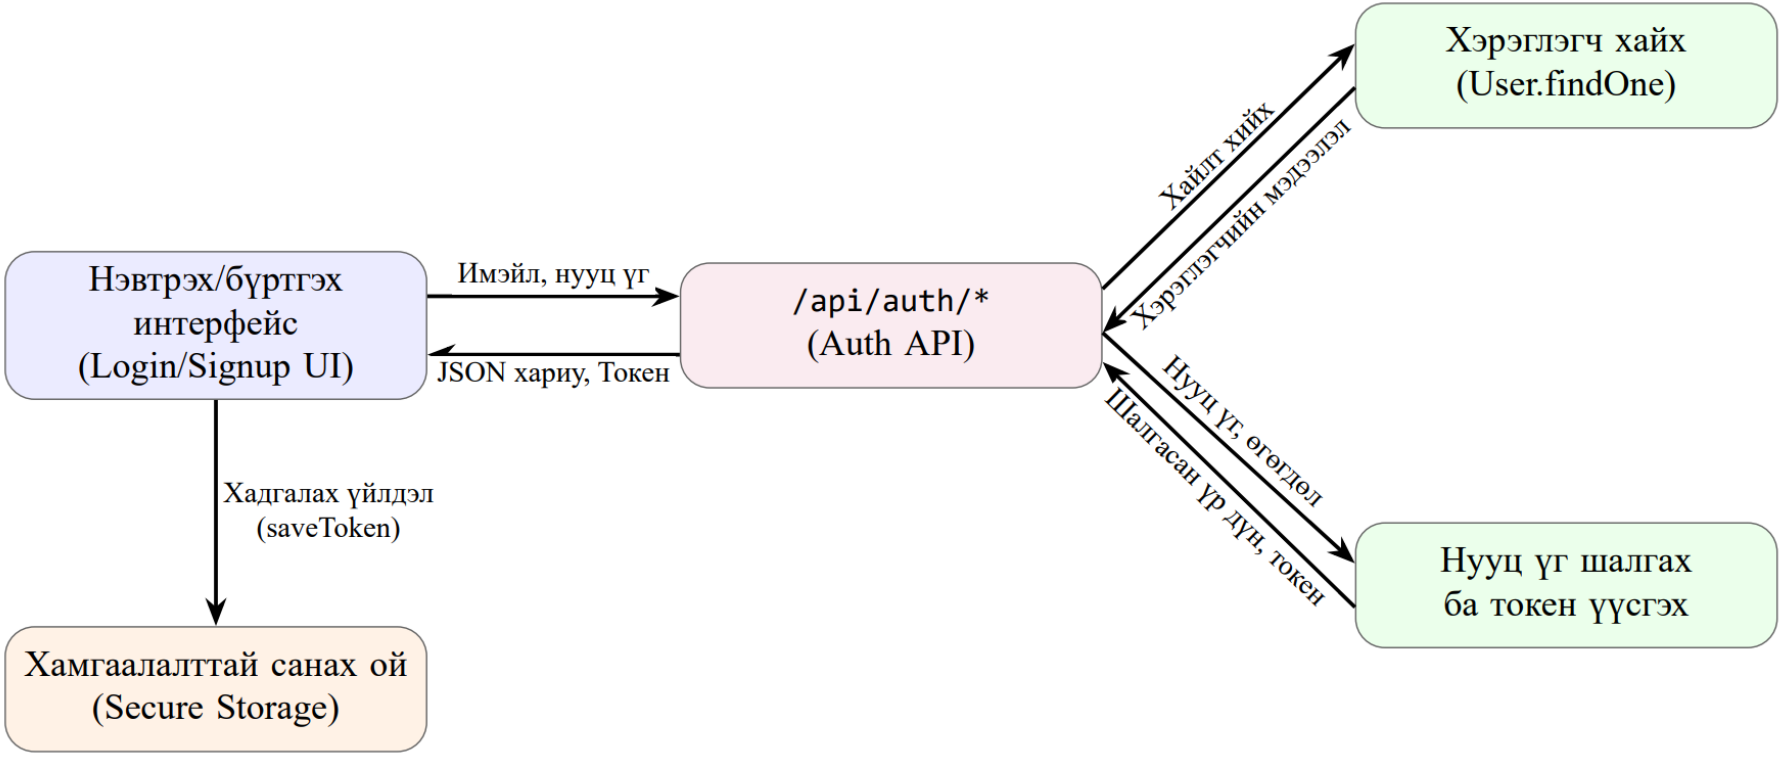
\includegraphics[width=0.95\textwidth]{Pictures/3,4.png}
\caption{Хоёрдугаар түвшний өгөгдлийн урсгал: нэвтрэх болон бүртгэх урсгал}
\label{fig:dfd_auth_detail}
\end{figure}

\noindent \fref{fig:dfd_auth_detail}-д хэрэглэгчийн бүртгэл/нэвтрэлтийн хүсэлт серверт дамжиж, хэрэглэгчийн мэдээлэл шалгах, нууц үг баталгаажуулах, JWT токен үүсгэх, токентой хариу буцаах дарааллыг өгөгдлийн урсгалын түвшинд дэлгэрүүлэн үзүүлэв.

\subsection{Тэмдэглэлийн CRUD урсгалын өгөгдлийн зураг}

\begin{figure}[H]
\centering
\makebox[\textwidth][c]{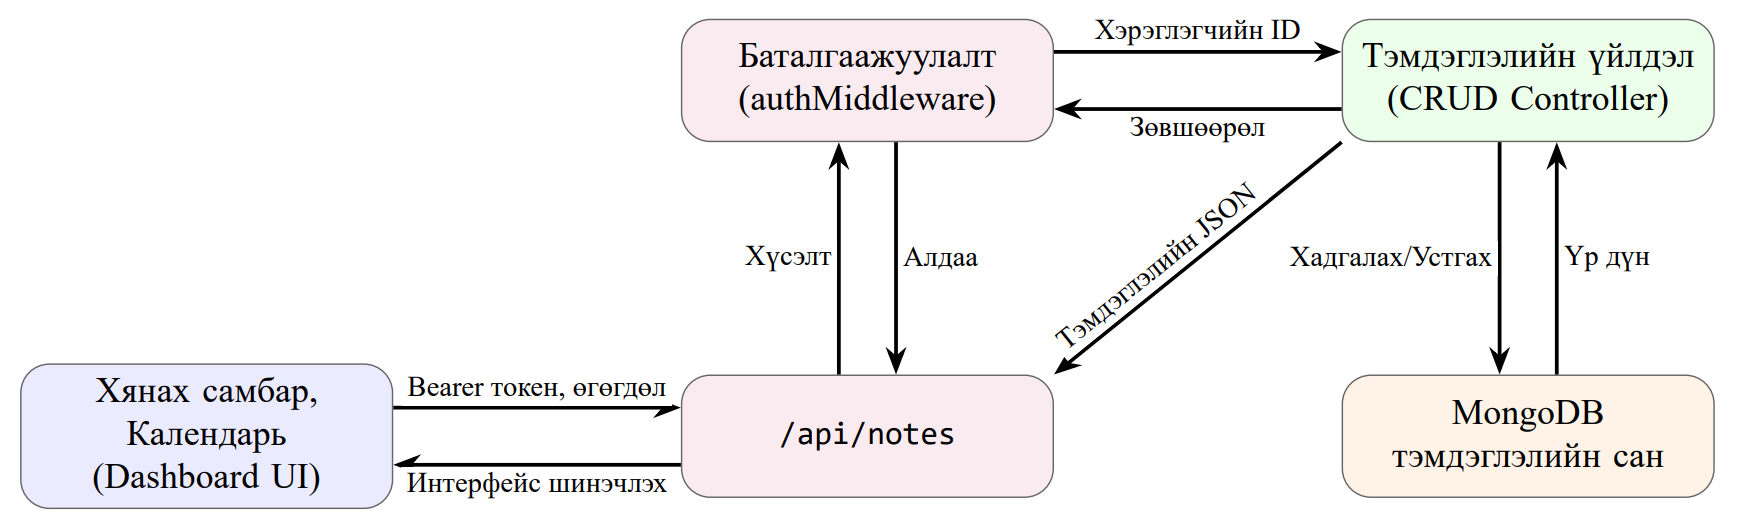
\includegraphics[width=0.98\textwidth]{Pictures/2r_tuvshin_3.png}}
\caption{Хоёрдугаар түвшний өгөгдлийн урсгал: тэмдэглэлийн CRUD урсгал}
\label{fig:dfd_notes_detail}
\end{figure}

\noindent \fref{fig:dfd_notes_detail}-д хэрэглэгчийн тэмдэглэлтэй холбоотой CRUD үйлдлийн өгөгдлийн урсгалыг харуулсан. Хэрэглэгчийн интерфейсээс илгээсэн хүсэлт \texttt{/api/notes} endpoint-оор дамжин эхлээд баталгаажуулалтын завсрын модульд (authentication middleware) шалгагдаж, зөвшөөрөгдсөн тохиолдолд хянагч модуль (controller) руу шилжин MongoDB мэдээллийн санд хадгалах, унших, шинэчлэх, устгах үйлдлүүдийг гүйцэтгэнэ.

\subsection{Стикер үүсгэх урсгалын өгөгдлийн зураг}

\begin{figure}[H]
\centering
\makebox[\textwidth][c]{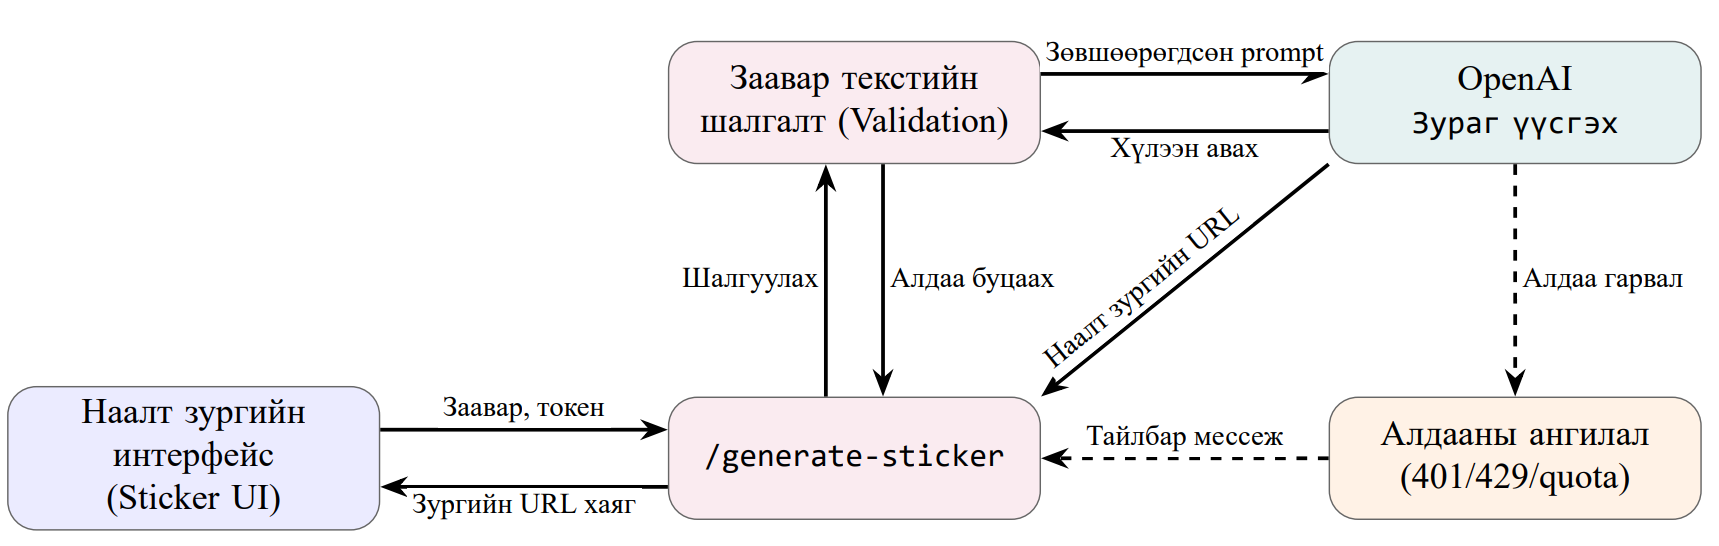
\includegraphics[width=0.98\textwidth]{Pictures/2r_tuvshin4.png}}
\caption{Хоёрдугаар түвшний өгөгдлийн урсгал: хиймэл оюун ухаанаар стикер үүсгэх урсгал (AI sticker generation)}
\label{fig:dfd_sticker_detail}
\end{figure}

\noindent \fref{fig:dfd_sticker_detail}-д хиймэл оюунд суурилсан стикер үүсгэх урсгалыг үзүүлсэн. Хэрэглэгчийн хүсэлт \texttt{/api/notes/generate-sticker} endpoint-оор орж, заавар текстийн шалгалтаар (validation) баталгаажсаны дараа OpenRouter API руу дамжуулан зураг үүсгэж, стикерийн холбоосыг клиент талд буцаах замналаар загварчлав.

\subsection{Өгөгдлийн урсгалын диаграммын тайлбар ба нэгтгэл}

Өгөгдлийн урсгалын диаграмм (DFD)-ыг энэ судалгаанд системийн логикийг шаталсан түвшинд ойлгомжтой тайлбарлах зорилгоор ашигласан. Диаграммын үндсэн тэмдэглэгээг дараах байдлаар хэрэглэв:

\begin{itemize}
    \item \textbf{Гаднах оролцогч (External entity):} системээс гадуурх хэрэглэгч эсвэл үйлчилгээ;
    \item \textbf{Процесс (Process):} өгөгдөл боловсруулж дараагийн шат руу шилжүүлдэг дотоод модуль;
    \item \textbf{Өгөгдлийн сан (Data store):} тогтмол хадгалалт хийгдэх мэдээллийн цэг;
    \item \textbf{Өгөгдлийн урсгал (Data flow):} модулиудын хооронд дамжих хүсэлт, хариу, бизнес өгөгдөл.
\end{itemize}

\begin{table}[H]
\centering
\caption{Өгөгдлийн урсгалын диаграммын түвшинчилсэн тайлбарын нэгтгэл}
\label{tab:dfd_explanation_summary}
\small
\setlength{\tabcolsep}{4pt}
\renewcommand{\arraystretch}{1.15}
\begin{tabularx}{\textwidth}{>{\raggedright\arraybackslash}p{2.2cm}>{\raggedright\arraybackslash}p{3.2cm}>{\raggedright\arraybackslash}X>{\raggedright\arraybackslash}p{2.4cm}}
\toprule
\textbf{Түвшин} & \textbf{Гол урсгал} & \textbf{Тайлбар} & \textbf{Зорилго} \\
\midrule
Контекст (Зураг 4.2) & Систем ба гадаад орчин & Хэрэглэгчийн UI хүсэлт системд орж, систем MongoDB болон OpenRouter API-тай өгөгдөл солилцох ерөнхий урсгалыг харуулсан. & Системийн хил хязгаар тодорхойлох \\
Нэгдүгээр түвшин (Зураг 4.3) & P1 Auth, P2 Notes, P3 Sticker & Контекст түвшний нэг процессыг баталгаажуулалт, тэмдэглэлийн CRUD, AI стикерийн модулиудад задалж, өгөгдлийн сан/гадаад үйлчилгээтэй харилцах логикийг харуулсан. & Архитектурын модульчилсан задаргаа \\
Хоёрдугаар түвшин (Зураг 4.4) & Нэвтрэх/бүртгэх урсгал & Хэрэглэгчийн бүртгэл, нэвтрэлт, нууц үгийн шалгалт, JWT токен үүсэлт ба хариу өгөгдлийн урсгалыг дэлгэрүүлсэн. & Auth урсгал баталгаажуулах \\
Хоёрдугаар түвшин (Зураг 4.5--4.6) & CRUD, Sticker урсгал & Тэмдэглэлийн CRUD болон AI стикер үүсгэх урсгалыг endpoint түвшинд нарийвчлан үзүүлсэн. & Гол бизнес урсгал баталгаажуулах \\
\bottomrule
\end{tabularx}
\normalsize
\end{table}

Ийнхүү DFD-ийг контекстээс нарийвчилсан түвшин рүү буулгаснаар системийн өгөгдөл дамжих дараалал, хариуцлагын зааг, баталгаажуулалтын цэгүүдийг судалгааны бичвэрт нотолгоотойгоор тайлбарлах боломж бүрдсэн.

\section{Дарааллын диаграммууд (sequence diagrams)}

Өгөгдлийн урсгалын зураг (dataflow) нь өгөгдөл хаашаа урсаж байгааг харуулдаг бол дарааллын диаграмм (sequence diagram) нь \textbf{цаг хугацааны дараалал}-ыг тодорхой харуулдаг. Энэ ажлын үндсэн гурван урсгалд дарааллын диаграмм (sequence diagram) ашиглав.

\subsection{Дарааллын диаграмм 1: Нэвтрэх урсгал}

\begin{figure}[H]
\centering
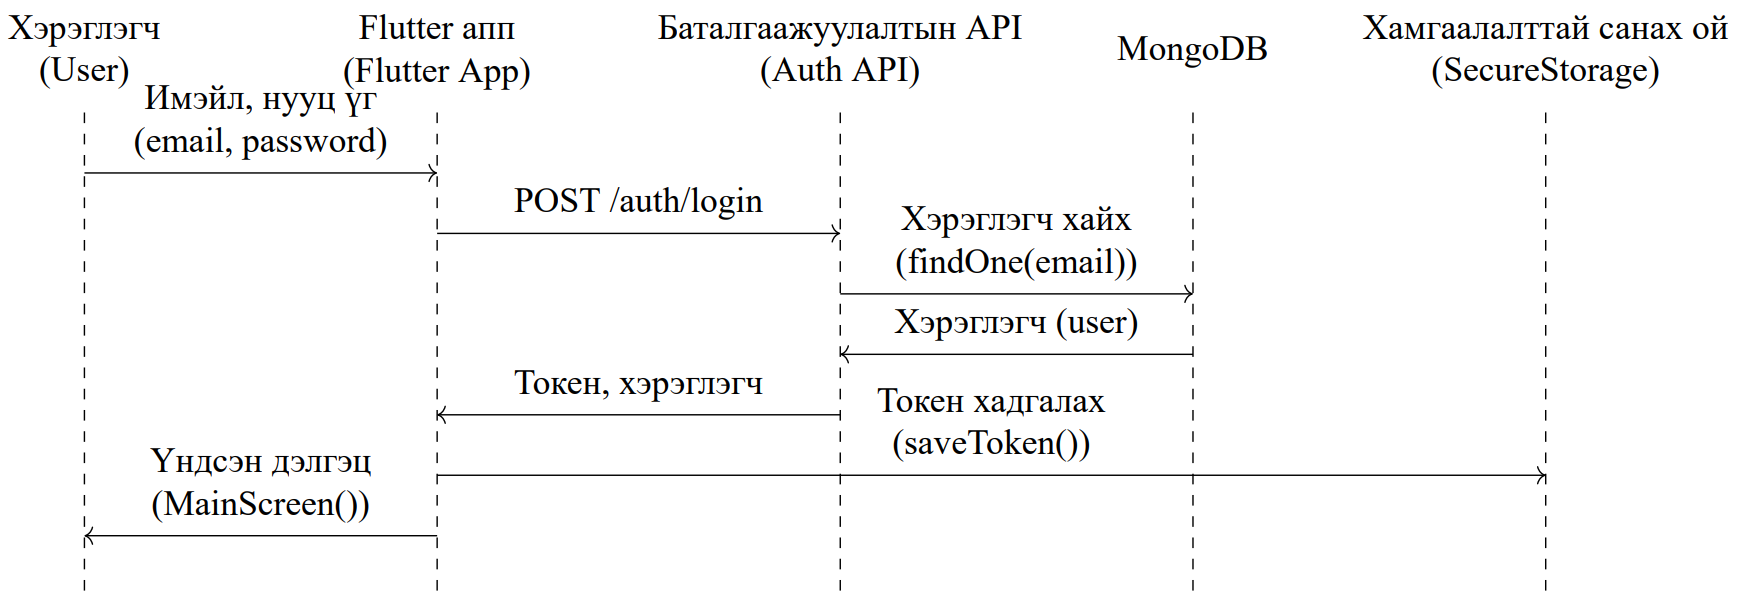
\includegraphics[width=0.95\textwidth]{Pictures/nevtreh1.png}
\caption{Дарааллын диаграмм: нэвтрэх урсгал}
\label{fig:seq_login}
\end{figure}

\noindent \fref{fig:seq_login}-д хэрэглэгч нэвтрэх мэдээллээ илгээснээс эхлэн сервер талд хэрэглэгч шалгах, нууц үг баталгаажуулах, JWT токен үүсгэх, улмаар апп талд токен хадгалж үндсэн дэлгэц рүү шилжих хүртэлх хугацааны дарааллыг харуулсан.

\subsection{Дарааллын диаграмм 2: Тэмдэглэл үүсгэх урсгал}

\begin{figure}[H]
\centering
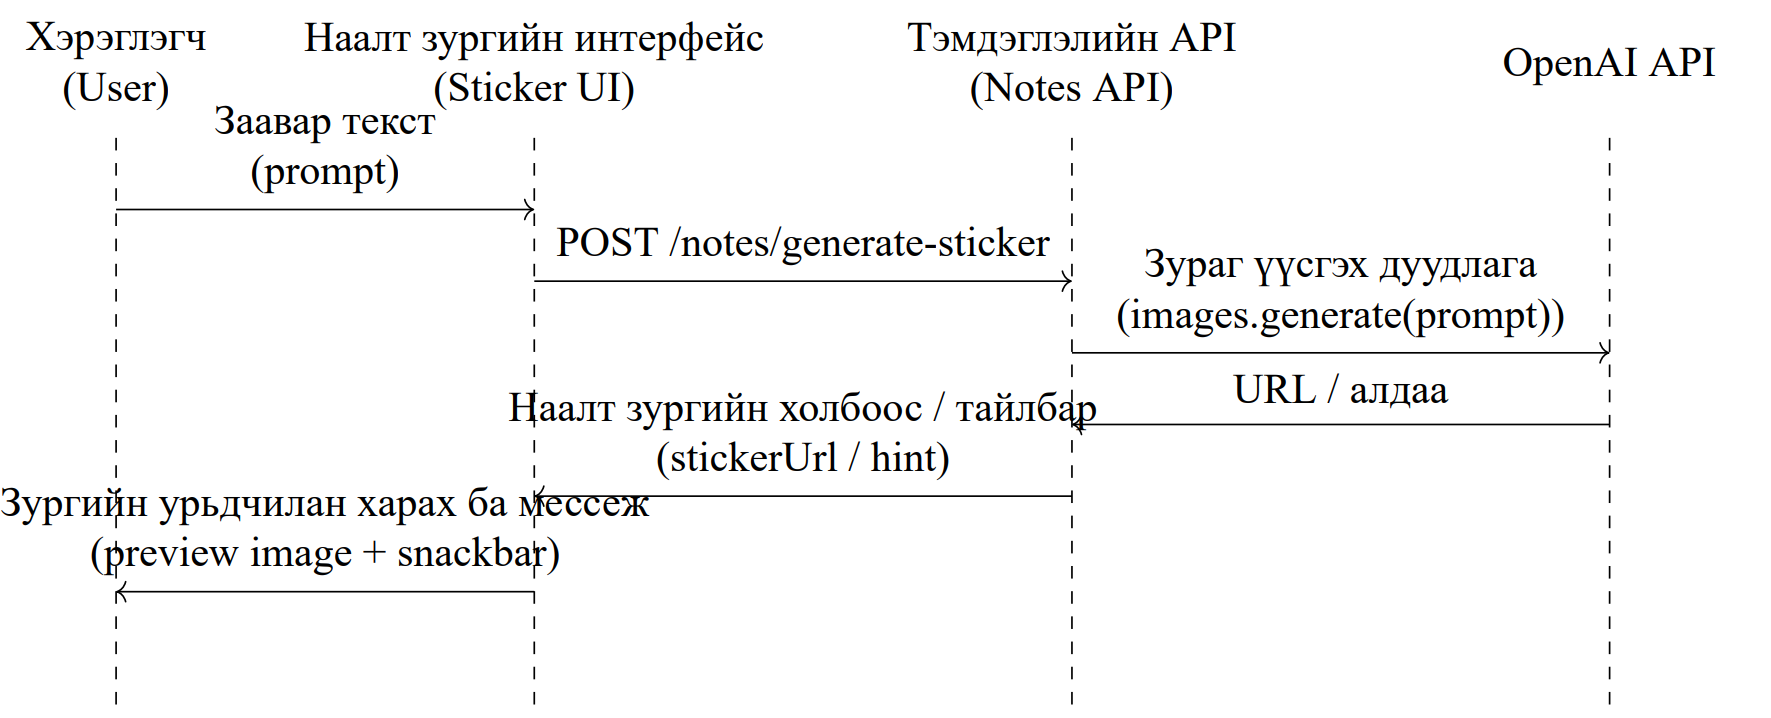
\includegraphics[width=0.95\textwidth]{Pictures/nevtreh3.png}
\caption{Дарааллын диаграмм: тэмдэглэл үүсгэх урсгал}
\label{fig:seq_note_create}
\end{figure}

\noindent \fref{fig:seq_note_create}-д шинэ тэмдэглэл үүсгэх хүсэлт токеноор баталгаажсаны дараа серверт хадгалагдаж, хариу өгөгдөл клиент талд ирэхэд жагсаалт болон интерфейсийн төлөв шинэчлэгдэх үе шат бүрийг дарааллаар нь үзүүлэв.

\subsection{Дарааллын диаграмм 3: Хиймэл оюун ухаанаар стикер үүсгэх урсгал (AI sticker generation)}

\begin{figure}[H]
\centering
\begin{tikzpicture}[
    font=\small,
    every node/.style={align=center},
    lbl/.style={fill=white, inner sep=1.2pt, font=\scriptsize}
]
\node at (0,0) {Хэрэглэгч\\(User)};
\node at (4,0) {стикерийн интерфейс\\(Sticker UI)};
\node at (8,0) {Тэмдэглэлийн API\\(Notes API)};
\node at (12,0) {OpenRouter API};

\foreach \x in {0,4,8,12} {\draw[dashed] (\x,-0.4) -- (\x,-6.0);} 

\draw[->] (0,-1.1) -- node[above, lbl] {Заавар текст\\(prompt)} (4,-1.1);
\draw[->] (4,-1.9) -- node[above, lbl] {POST /notes\\generate-sticker} (8,-1.9);
\draw[->] (8,-2.7) -- node[above, lbl] {Зураг үүсгэх\\дуудлага\\images.generate(prompt)} (12,-2.7);
\draw[->] (12,-3.5) -- node[above, lbl] {URL / алдаа} (8,-3.5);
\draw[->] (8,-4.3) -- node[above, lbl] {стикерийн холбоос\\(stickerUrl / hint)} (4,-4.3);
\draw[->] (4,-5.1) -- node[above, lbl] {Урьдчилан харах ба мессеж\\(preview + snackbar)} (0,-5.1);
\end{tikzpicture}
\caption{Дарааллын диаграмм: хиймэл оюун ухаанаар стикер үүсгэх урсгал (AI sticker generation)}
\label{fig:seq_sticker}
\end{figure}

\noindent \fref{fig:seq_sticker}-д заавар текст (prompt) клиентээс сервер рүү дамжин OpenRouter API үйлчилгээ дуудсаны дараа стикерийн URL эсвэл алдааны мэдээлэл буцаж, хэрэглэгчид урьдчилан харах болон мессеж хэлбэрээр хүрэх логикийг хугацааны тэнхлэгээр дүрсэлсэн.

\section{Хэрэглээний тохиолдлын загвар (Use Case Diagram)}

Хэрэглээний тохиолдлын диаграмм (use case diagram) нь системийн функционал хил хязгаар (system boundary) болон хэрэглэгчийн оролцооны үүргийг ерөнхий түвшинд тодорхойлох зорилготой. Энэ нь өгөгдлийн урсгал (dataflow) ба дарааллын диаграмм (sequence diagram)-ын өмнөх ойлголтын гүүр болж, хэрэглэгч системтэй яг ямар зорилгоор харилцаж байгааг нэг зурагт нэгтгэн харуулдаг.

Энэхүү судалгаанд үндсэн оролцогчоор эцсийн хэрэглэгч (mobile user)-ийг авч үзэж, нэвтрэх/бүртгэх, тэмдэглэл удирдах, календарь харах, стикер үүсгэх, сануулга-мэдэгдэлтэй ажиллах гэсэн гол хэрэглээний тохиолдлуудыг загварчилсан.

\begin{figure}[H]
\centering
\resizebox{0.9\textwidth}{!}{%
\begin{tikzpicture}[
    font=\small,
    uc/.style={ellipse, draw=purple!70, fill=purple!8, minimum width=8.1cm, minimum height=1.1cm, align=center},
    actorlbl/.style={font=\small}
]

% Actor (stick figure)
\coordinate (ah) at (-7.8,2.2);
\draw[thick] (ah) circle (0.35);
\draw[thick] (-7.8,1.85) -- (-7.8,0.75);
\draw[thick] (-8.4,1.4) -- (-7.2,1.4);
\draw[thick] (-7.8,0.75) -- (-8.25,-0.2);
\draw[thick] (-7.8,0.75) -- (-7.35,-0.2);
\node[actorlbl] at (-7.8,-0.6) {Хэрэглэгч};

% System boundary
\draw[rounded corners=10pt, thick, draw=blue!60] (-5.4,-4.0) rectangle (8.8,4.0);
\node[anchor=north west, font=\bfseries\small] at (-5.2,3.8) {AI Notebook систем};

% Use cases
\node[uc] (ucAuth) at (1.7,2.9) {Бүртгэх / Нэвтрэх};
\node[uc] (ucNotes) at (1.7,1.4) {Тэмдэглэл үүсгэх, засах, устгах};
\node[uc] (ucCalendar) at (1.7,-0.1) {Календарь дээрээс тэмдэглэл харах};
\node[uc] (ucSticker) at (1.7,-1.6) {Хиймэл оюун ухаанаар стикер үүсгэх};
\node[uc] (ucNotif) at (1.7,-3.1) {Сануулга тохируулах, мэдэгдэл харах};

% Associations
\draw[thick] (-7.2,1.4) -- (ucAuth.west);
\draw[thick] (-7.2,1.4) -- (ucNotes.west);
\draw[thick] (-7.2,1.4) -- (ucCalendar.west);
\draw[thick] (-7.2,1.4) -- (ucSticker.west);
\draw[thick] (-7.2,1.4) -- (ucNotif.west);

\end{tikzpicture}%
}
\caption{AI Notebook системийн хэрэглээний тохиолдлын диаграмм}
\label{fig:usecase_overview}
\end{figure}

\section{Өгөгдлийн сангийн ER диаграмм (Entity-Relationship Diagram)}

Энэ хэсэгт AI Notebook системийн өгөгдлийн бүтэц болон entity хоорондын хамаарлыг харуулав. Үндсэн тэмдэглэгээний хэлбэр нь \texttt{||-->} бөгөөд энд \texttt{||} = яг нэг (mandatory one), \texttt{>} = олон (many) гэсэн утгатай.

\begin{figure}[H]
\centering
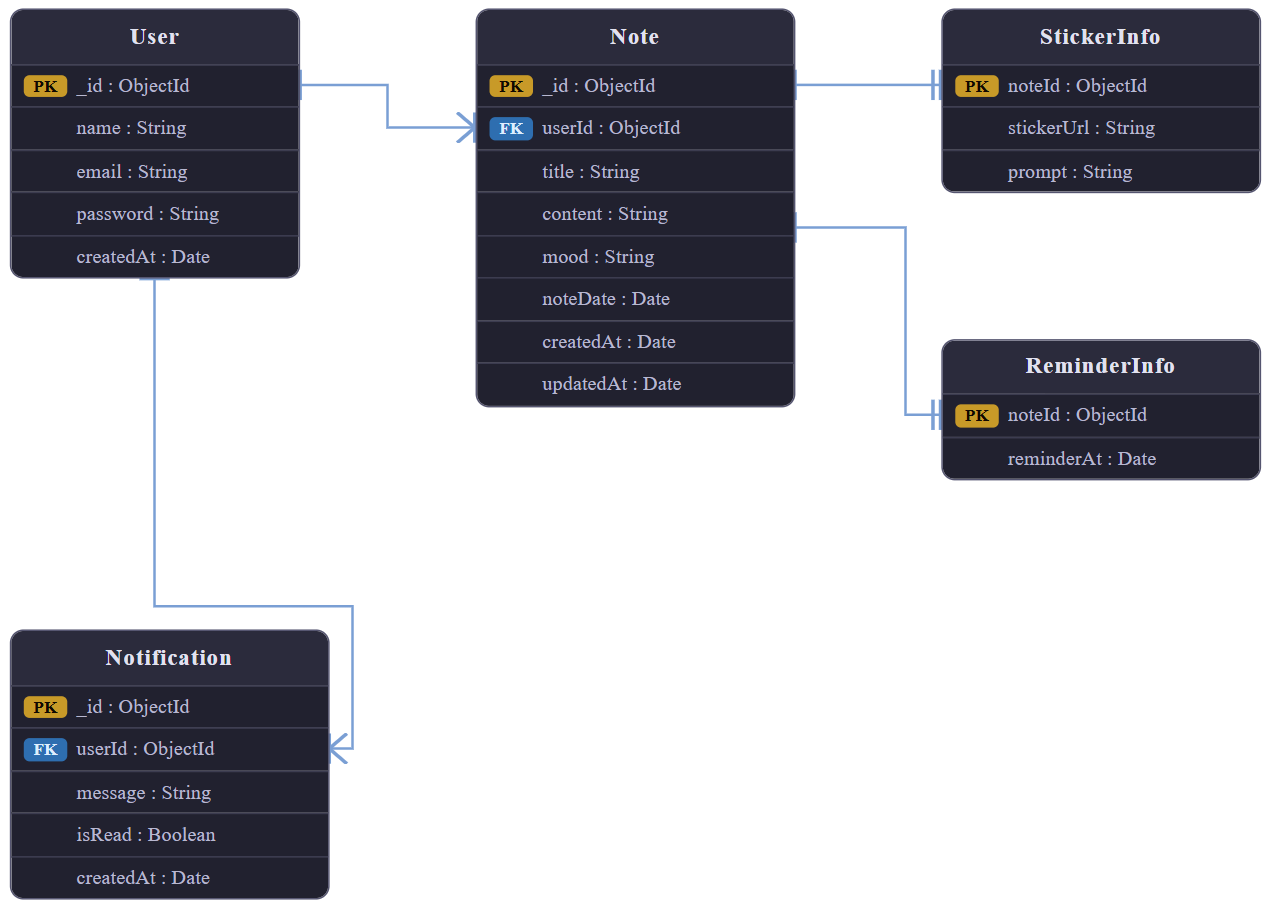
\includegraphics[width=0.98\textwidth]{Pictures/ERD.png}
\caption{AI Notebook системийн өгөгдлийн сангийн ER диаграммын задаргаа}
\label{fig:erd_overview}
\end{figure}

\noindent \fref{fig:erd_overview}-ийн харилцааны утга нь дараах байдалтай.

\begin{itemize}
    \item \texttt{User ||-> Note}: нэг хэрэглэгч олон тэмдэглэлтэй.
    \item \texttt{Note ||--|| StickerInfo}: нэг тэмдэглэлд нэг стикерийн мэдээлэл холбогдоно (логикийн хувьд \texttt{0..1} буюу optional).
    \item \texttt{Note ||--|| ReminderInfo}: нэг тэмдэглэлд нэг сануулгын мэдээлэл холбогдоно (логикийн хувьд \texttt{0..1} буюу optional).
    \item \texttt{User ||-> Notification}: нэг хэрэглэгч олон мэдэгдэл хүлээн авна.
\end{itemize}

\noindent PK/FK-ийн товч тайлбар:

\begin{itemize}
    \item \textbf{PK (Primary Key)}: хүснэгтийн мөр бүрийг давтагдашгүй таних үндсэн түлхүүр. Жишээ нь \texttt{User.\_id}, \texttt{Note.\_id}.
    \item \textbf{FK (Foreign Key)}: өөр entity-ийн PK-руу заасан холбоос түлхүүр. Жишээ нь \texttt{Note.userId $\rightarrow$ User.\_id}. Энэ холбоосоор тэмдэглэл аль хэрэглэгчтэй хамаарахыг тогтооно.
\end{itemize}

\noindent Тайлбар: концепцийн ERD дээр \texttt{StickerInfo} ба \texttt{ReminderInfo}-г тусдаа entity хэлбэрээр үзүүлсэн. Харин бодит MongoDB хэрэгжилтэд эдгээр нь \texttt{Note} document доторх \texttt{stickerUrl} болон \texttt{reminderAt} nullable талбаруудаар хадгалагдана.

\section{Шалгуур}

Системийн урсгал бүрийг дараах шалгуураар баталгаажуулсан:

\begin{itemize}
    \item Баталгаажуулалтын урсгал (auth flow): токен олголт, хадгалалт, дэлгэц шилжилтийн (navigation) зөв байдал;
    \item Тэмдэглэлийн урсгал (notes flow): CRUD үйлдлийн дараах өгөгдлийн тууштай байдал;
    \item стикерийн урсгал (sticker flow): заавар текстээс (prompt) URL буцах, алдааны тайлбар зөв харуулах эсэх;
    \item Мэдэгдлийн урсгал (notification flow): сануулгыг зөв хуваарьлах/цуцлах, мэдэгдлийн жагсаалтын төлөв шинэчлэх;
    \item Аюулгүй байдлын урсгал (security flow): токенгүй хүсэлтэд 401 буцах эсэх.
\end{itemize}

\section{Generative AI туршилтын аргачлал}

Энэхүү судалгаанд хиймэл оюун ухаанд суурилсан \texttt{/api/notes/generate-sticker} төгсгөлийн цэгийг (endpoint) бодит орчинд шалгаж, үр дүнг зөвхөн дараах хоёр метрикаар үнэлэв.

\begin{enumerate}
    \item \textbf{Latency} (зураг үүсгэх хугацаа, секунд),
    \item \textbf{Prompt relevance} (үсгэсэн зураг prompt-той нийцэж байгаа эсэх).
\end{enumerate}

Туршилтыг 2026-04-17-нд Windows орчинд ажилласан Node.js backend дээр хийж, баталгаажуулалтын (JWT) токентой хүсэлтүүдийг \texttt{Invoke-RestMethod} ашиглан давтан илгээсэн.

\subsection*{Latency хэмжих арга}

Хүсэлт бүрийн эхлэх ба дуусах хугацааг тэмдэглэж, зураг үүсгэх хугацааг секундээр тооцов:
\begin{equation}
\label{eq:latency}
t_{\mathrm{latency}} = t_{\mathrm{response}} - t_{\mathrm{request}}\; (\mathrm{sec})
\end{equation}

Нэг сценар доторх дундаж хугацааг:
\begin{equation}
\label{eq:mean_latency}
\overline{t} = \frac{1}{N}\sum_{i=1}^{N} t_i
\end{equation}
томьёогоор гаргав.

\subsection*{Generative AI туршилтын сценарийн дефиниц}

Generative AI гүйцэтгэлийг үнэлэхийн тулд OpenRouter fallback стратегийн өөр өөр сценарийг туршив:

\begin{itemize}
    \item \textbf{S1 (Internal fallback, unique prompt)}: Уникаль prompt бүрэлмж ашиглаж, гаднын OpenRouter үйлчилгээ суугдахгүйгээр дотоод fallback (cached sticker templates) ашигласан. $N=40$ давтуулгаар дотоод механизмын үр ашиг, CPU ачаалалыг хэмжив. Хүлээгдсэн үр дүн: хамгийн бага latency, тогтвортой performance.
    
    \item \textbf{S2 (Designed fallback, unique prompt, network latency)}: Уникаль prompt-ыг OpenRouter рүү дамжүүлэх үед сүлжээний саатлыг симуляцлаж ($N=10$ давтуулга), OpenRouter амжилтгүй болох үед system дотоод fallback руу шилжихийн үр дүнг хэмжив. Энэ сценарт ambiguous/complex prompt-уудыг ашигласан. Хүлээгдсэн үр дүн: өндөр latency variation, fallback source-ийн сонголт, дараа дахь retry стратегийн үр нөлөө.
    
    \item \textbf{S3 (Designed fallback, cached prompt)}: Өмнө үүсгэн хадгалсан prompt-ыг давтан ашиглаж ($N=10$ давтуулга), кэшэ дэх өмнөх үр дүнг ашигласан. Хүлээгдсэн үр дүн: хамгийн бага latency, 100\% hit rate, caching механизмын үр ашиг.
\end{itemize}

\subsection*{Prompt relevance үнэлэх арга}

 Үүсгэсэн зураг бүрийг prompt-ийн үндсэн утгатай тохирч байгаа эсэхээр бинар үнэлэв:

\begin{itemize}
    \item \textbf{1 (нийцсэн)}: prompt-д өгсөн гол объект/үйлдэл зурагт тодорхой харагдсан,
    \item \textbf{0 (нийцээгүй)}: prompt-ийн гол утга алдагдсан эсвэл өөр сэдэв рүү хазайсан.
\end{itemize}

Нийцлийн хувийг дараах байдлаар тооцов:
\begin{equation}
\label{eq:prompt_relevance}
\text{Prompt relevance rate}(\%) = \frac{N_{\mathrm{match}}}{N_{\mathrm{total}}} \times 100
\end{equation}
энд $N_{match}$ нь нийцсэн зураг, $N_{total}$ нь нийт үүсгэсэн зураг болно.

\section{Туршилтын протокол ба өгөгдөл цуглуулах зохион байгуулалт}

Энэхүү судалгаанд туршилтыг "бэлтгэл -- гүйцэтгэл -- баталгаажуулалт -- бүртгэл" гэсэн дөрвөн үе шаттай протоколоор хийсэн. Протоколчилсон шалтгаан нь туршилтын давтагдахуйц чанарыг (reproducibility) нэмэгдүүлж, хэмжилтийн ялгааг орчны санамсаргүй нөлөөнөөс тусгаарлах явдал юм.

\begin{enumerate}
    \item \textbf{Бэлтгэл:} backend орчны хувьсагч (JWT, database, OpenRouter key), тест хэрэглэгч, үндсэн датаг ижил нөхцөлөөр бэлдэх;
    \item \textbf{Гүйцэтгэл:} сценар тус бүрт ижил payload, ижил endpoint дараалал ашиглах;
    \item \textbf{Баталгаажуулалт:} HTTP статус, response body, UI төлөв, өгөгдлийн сангийн үр дүнг зэрэг шалгах;
    \item \textbf{Бүртгэл:} latency, алдаа, fallback эх үүсвэр, CPU ажиглалтыг нэг загвараар тэмдэглэх.
\end{enumerate}

\begin{table}[H]
\centering
\caption{Туршилтын протоколын нэгтгэл}
\label{tab:test_protocol_summary}
\small
\setlength{\tabcolsep}{4pt}
\renewcommand{\arraystretch}{1.15}
\begin{tabularx}{\textwidth}{>{\raggedright\arraybackslash}p{2.0cm}>{\raggedright\arraybackslash}X>{\raggedright\arraybackslash}p{3.0cm}>{\raggedright\arraybackslash}p{2.4cm}}
\toprule
\textbf{Сценар} & \textbf{Товч тодорхойлолт} & \textbf{Гол хэмжилт} & \textbf{Хүлээгдсэн үр дүн} \\
\midrule
AUTH-01 & Зөв credential-ээр нэвтрэх & HTTP 200, token field & Амжилттай нэвтрэлт \\
AUTH-02 & Токенгүй хамгаалалттай endpoint дуудах & HTTP 401 & Хандалт хориглогдох \\
CRUD-01 & Тэмдэглэл үүсгэх/засах/устгах дараалал & DB change + UI refresh & Өгөгдлийн тууштай байдал \\
AI-01 & Уникаль prompt-оор стикер үүсгэх & Latency, response source & URL эсвэл fallback хариу \\
AI-02 & Давтагдсан prompt урсгал & Latency variation, cache/fallback behavior & Тогтвортой response хэв шинж \\
NOTIF-01 & Reminder тохируулах ба хүргэх & Trigger time, notification event & Хугацаанд нийцсэн мэдэгдэл \\
\bottomrule
\end{tabularx}
\normalsize
\end{table}

Өгөгдөл цуглуулахдаа хэмжилтийн бүртгэлийг нэг форматаар хадгалж, алдааны тохиолдолд endpoint, payload төрөл, хариу код, fallback эх үүсвэрийг тусад нь тэмдэглэсэн. Ийнхүү структурчилсан бүртгэл нь үр дүнг дараа нь бүлэглэж шинжлэх, орчны шалтгаант хэлбэлзлийг тайлбарлах боломжийг нэмэгдүүлсэн.

\section{Хүчин төгөлдөр байдлын эрсдэл ба бууруулах арга}

Судалгааны арга зүйн найдвартай байдлыг үнэлэхдээ дотоод (internal), гадаад (external), бүтэц-ойлголтын (construct) болон дүгнэлтийн (conclusion) хүчин төгөлдөр байдлын эрсдлийг ялган авч үзэв.

\begin{table}[H]
\centering
\caption{Хүчин төгөлдөр байдлын эрсдэл ба бууруулах стратеги}
\label{tab:validity_threats}
\small
\setlength{\tabcolsep}{4pt}
\renewcommand{\arraystretch}{1.15}
\begin{tabularx}{\textwidth}{>{\raggedright\arraybackslash}p{2.8cm}>{\raggedright\arraybackslash}X>{\raggedright\arraybackslash}p{3.9cm}}
\toprule
\textbf{Эрсдэлийн төрөл} & \textbf{Болзошгүй нөлөө} & \textbf{Бууруулах арга} \\
\midrule
Дотоод хүчин төгөлдөр байдал & Орчны тохиргоо өөрчлөгдвөл тестийн үр дүн зөрөх & Нэг орчинд ижил протоколоор давтан гүйцэтгэл хийх \\
Гадаад хүчин төгөлдөр байдал & Нэг хэрэглэгч/нэг төхөөрөмжийн дүн бүх хэрэглээнд шууд ерөнхийшөхгүй байх & Өөр сценар, өөр prompt багц ашиглан харьцуулсан үнэлгээ хийх \\
Construct validity & "Чанар" ойлголтыг буруу метрикаар төлөөлөх эрсдэл & Latency, статус код, UX feedback зэрэг олон индикатор хослуулах \\
Conclusion validity & Бага хэмжээний сорьц дээр хэт ерөнхий дүгнэлт хийх эрсдэл & p50/p95, mean, max зэрэг тархалтын үзүүлэлтээр тайлбарлах \\
\bottomrule
\end{tabularx}
\normalsize
\end{table}

Ийм эрсдэлийн шинжилгээг арга зүйн хэсэгт тусгаснаар судалгааны үр дүн нь зөвхөн эерэг кейсийн тайлбар бус, баталгаажуулалтын хязгаарлалтаа ил тод тэмдэглэсэн академик бүтцэд шилжиж байна.

